%!TEX root = main_ISMB.tex
\section{Results}
\label{sec:results}

\subsection{Implementation}
\label{sec:implementation}
Our software, \texttt{Incarnation}, was implemented in Python2.7. We used
\emph{RNAinverse} from the \textit{Vienna Package 2.0}~\cite{Hofacker:1994}.
All time benchmarks were run on a one AMD Opteron(tm) Processor 6278  at 2.4 GHz with cache of 512 KB.
 We used as parameter $\beta=15$, the penalty for an invalid base pair.



We present in Fig.~\ref{fig:time} the average times to generate one sequence
with the required \texttt{C+G} content. As expected, the time grows linearly
in function of the length of the structures.  A highly interesting feature
is the huge decrease in time of computation when there is $15\%$ free 
nucleotides inside the loops of the secondary structure.

\begin{figure}[ht!]
	\centering
	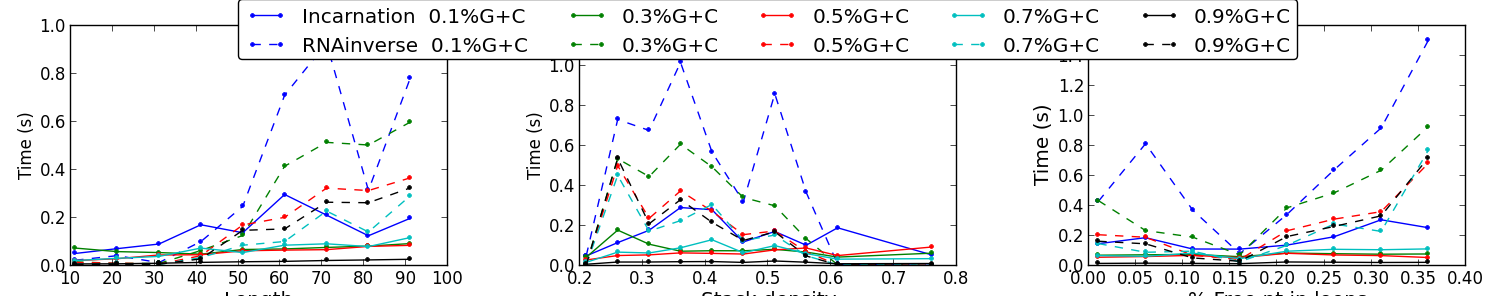
\includegraphics[scale=0.45]{Figures/time_rnastrand_clustered_rnainverse_100samples_fix}
	\caption{Average time in seconds to generate one sequence. We explicitly show 
	the time spent by \texttt{Incarnation} (full line) and \texttt{RNAinverse} (dashed) for various \texttt{C+G} contents. The first plot is in function
	of the length of the structures. The second is in function of the stack
	density (i.e. $2\cdot\#stacks/length$) and the latter in function of 
	the proportion of free nucleotides (i.e. not base paired) inside loops.}
	\label{fig:time}	
\end{figure}



\subsection{Dataset}
To evaluate the quality of our method, we selected a subset of $50$ secondary
structures from the \textit{RNA STRNAD} database~\cite{andronescu2008rna}.
Those are known secondary structure from a variety of organisms with 
 lengths between $20$ and $100$ nucleotides. 
 
 TODO MORE INFO RNASTRAND???
 
 To ease the visualization of the data, we clustered together the strucures
 in function of their length, stacks density and proportion of free 
 nucleotides in loops. We present in Fig.~\ref{fig:bins} the distribution
 of the structures in the different bins.
 
 \begin{figure}[ht!]
 	\centering
	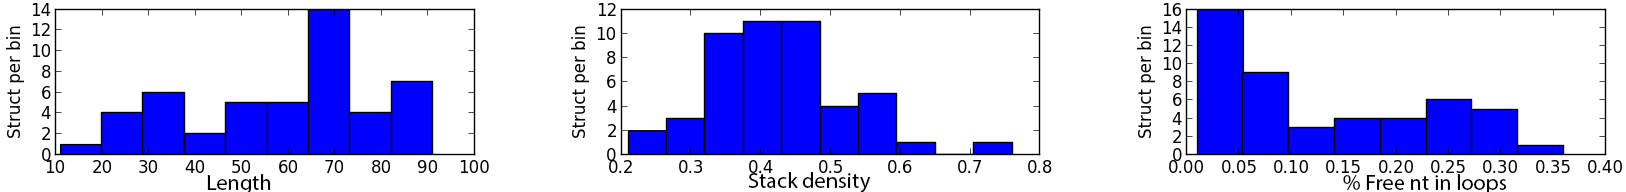
\includegraphics[scale=0.45]{Figures/bins_distribution.png}
	\caption{Number of secondary structures per bins.}
	\label{fig:bins}
 \end{figure}
 
 
\subsection{Design}
 To benchmark our method, we first started by sampling a minimum
 $100$ sequence per structures. After correcting the free nucleotides with
 \texttt{RNAinverse} we computed their MFE with \texttt{RNAfold} from the \textit{Vienna Package 2.0}~\cite{Hofacker:1994}.
 
A first criterion is which percentage of sequences have as MFE the target
secondary structures. We are also interested by the number of structures
for which we can design at least one sequence with the desired MFE.
We show the results when using only \texttt{Incarnation} in 
 Fig.~\ref{fig:mfe_struct_solved_noinverse}. The high rate of failure
is due to the fact that no selection criterions are applied to
free nucleotides. A local strategy is thus needed.
After processing \texttt{Incarnation} sequences with \RNAinverse to 
locally optimize the free nucleotides, we obtain the results 
in Fig.~\ref{fig:mfe_struct_solved}. We observe
that length is not a good predictor for the quality of the results. Instead,
a high number of free nucleotides in the structure seems to be a 
good measure of its design hardness. 
On top of that, with a \texttt{C+G} content of $50\%$ and more, at least
one solutions was found for almost all structures. The difficulty of 
designing sequences for targets with a high number of free nucleotides 
 in loops appears clearly in the last subfigure. Even with a high \texttt{C+G} content a our method was not able to generate solutions for a few
 structures. 

\begin{figure}[ht!]	
	\centering
	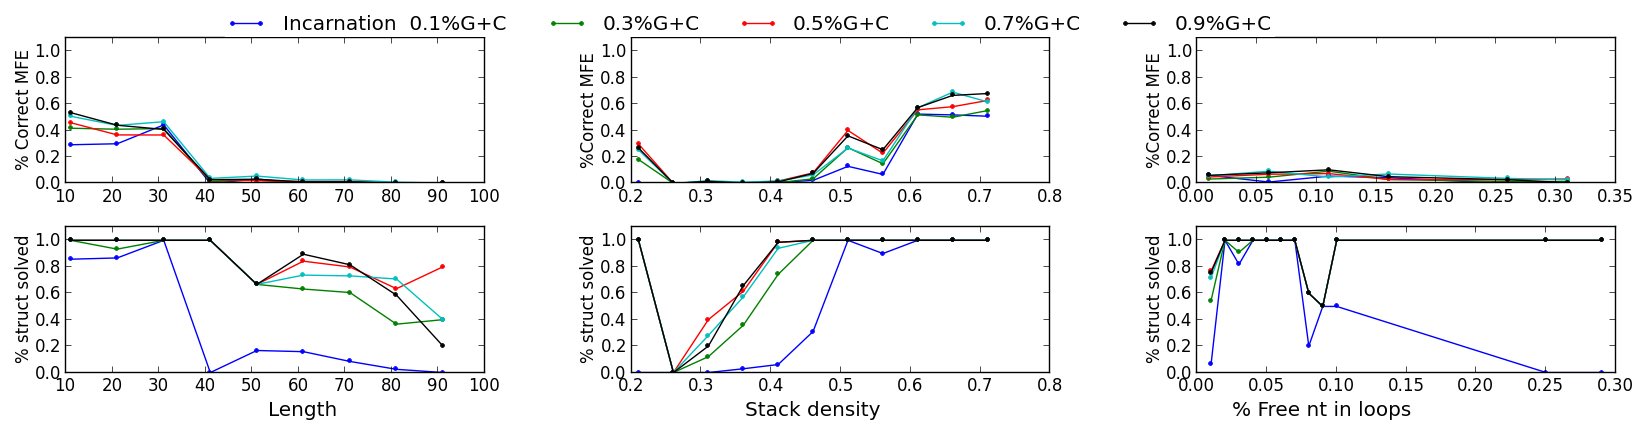
\includegraphics[scale=0.45]{Figures/mfe_struct_solve_nornainverse.png}
	\caption{Quality of \texttt{Incarnation} results. The first row shows the percentage
	of sampled sequences folding into the target. The second shows the 	
	proportion	of structures for which at least one correct sequence was 
	sampled.}
	\label{fig:mfe_struct_solved_noinverse}	
\end{figure}



\begin{figure}[ht!]	
	\centering
	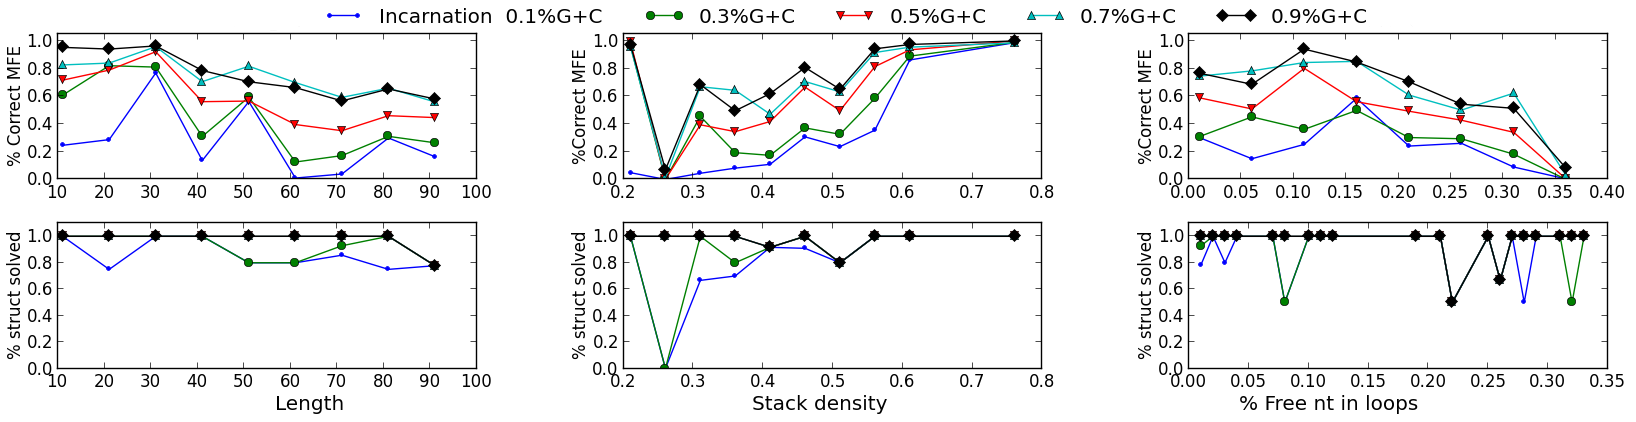
\includegraphics[scale=0.45]{Figures/mfe_struct_solved}
	\caption{Quality of \texttt{Incarnation+RNAinverse} results. The first row shows the percentage
	of sampled sequences folding into the target. The second shows the 	
	proportion	of structures for which at least one correct sequence was 
	sampled.}
	\label{fig:mfe_struct_solved}	
\end{figure}
 
To evaluate the global quality of \texttt{Incarnation} sequences, we show
in Fig.~\ref{fig:ss_sens} the ratio of well predicted base pairs in the
MFE structure of our sampled sequences. We can observe that, in all cases,
the hardest sequence to design are those with an extremely low \texttt{C+G}
content. As anticipated, those are the sequences with the weakest bonds.
We notice that the most accurate sequences yield a \texttt{C+G} content
of $70\pm 10\%$. 

As discussed in Sec.~\ref{sec:implementation}, we notice a highly decreased
computational time needed to generate the sequences with $15\%$ free 
nucleotides in the loops. We remark that those structures also yield 
a much lower structural sensitivity.

\begin{figure}[ht!]
 	\centering
	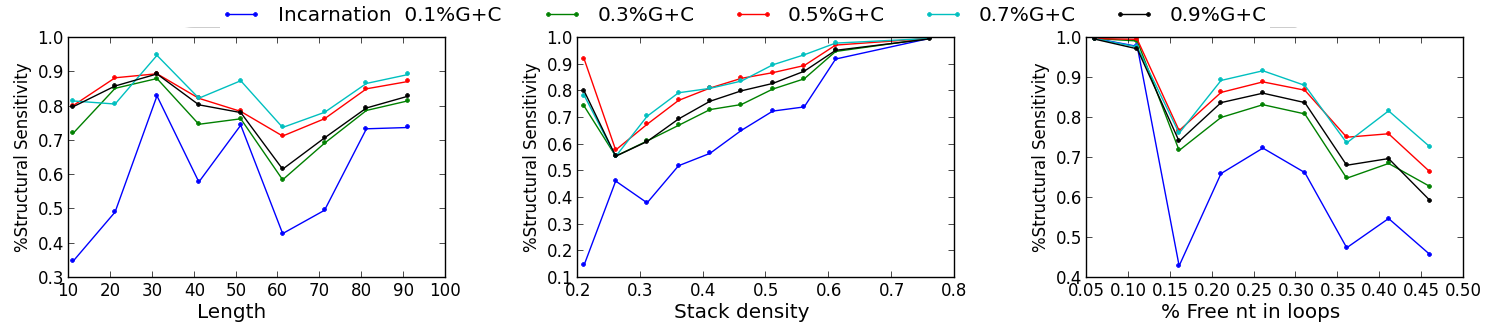
\includegraphics[scale=0.45]{Figures/rnastrand_clustered_rnainverse_100samples_struct_sens.png}
	\caption{Structural sensitivity (i.e. $\#$ well predicted base pairs / $\#$ base pairs in target) of the sampled sequences MFE. }
	\label{fig:ss_sens}	
\end{figure}


\subsection{Samples properties}

In this section, we are only interested  in the samples folding into the 
targetMFE. 

A desirable feature in sequence design, is to produce samples with a high
diversity. We show in Fig.~\ref{fig:nb_sols_entropy} the number of correct
solutions as their average entropy and base pair entropy, since 
\texttt{Incarnation}  only influences the distribution of nucleotides inside 
stacked base pairs. The most constraining factor for generating valid
 solutions seems to be  low \texttt{C+G} content and the percentage of free nucleotides. Our method is able to generate 

Also, a critical properties in RNA sequence design is 
the frequency of the MFE. 
The sequence should be in its target conformation long enough to
perform the desired action. Presented in Fig.~\ref{fig:freq} we see that
there is a slow decline of the frequency with the increase in size. Yet,
for an average \texttt{C+G} content, the frequency stays over $10\%$ even
at size of $100$ nucleotides.


\begin{figure}[ht!]
	\centering
	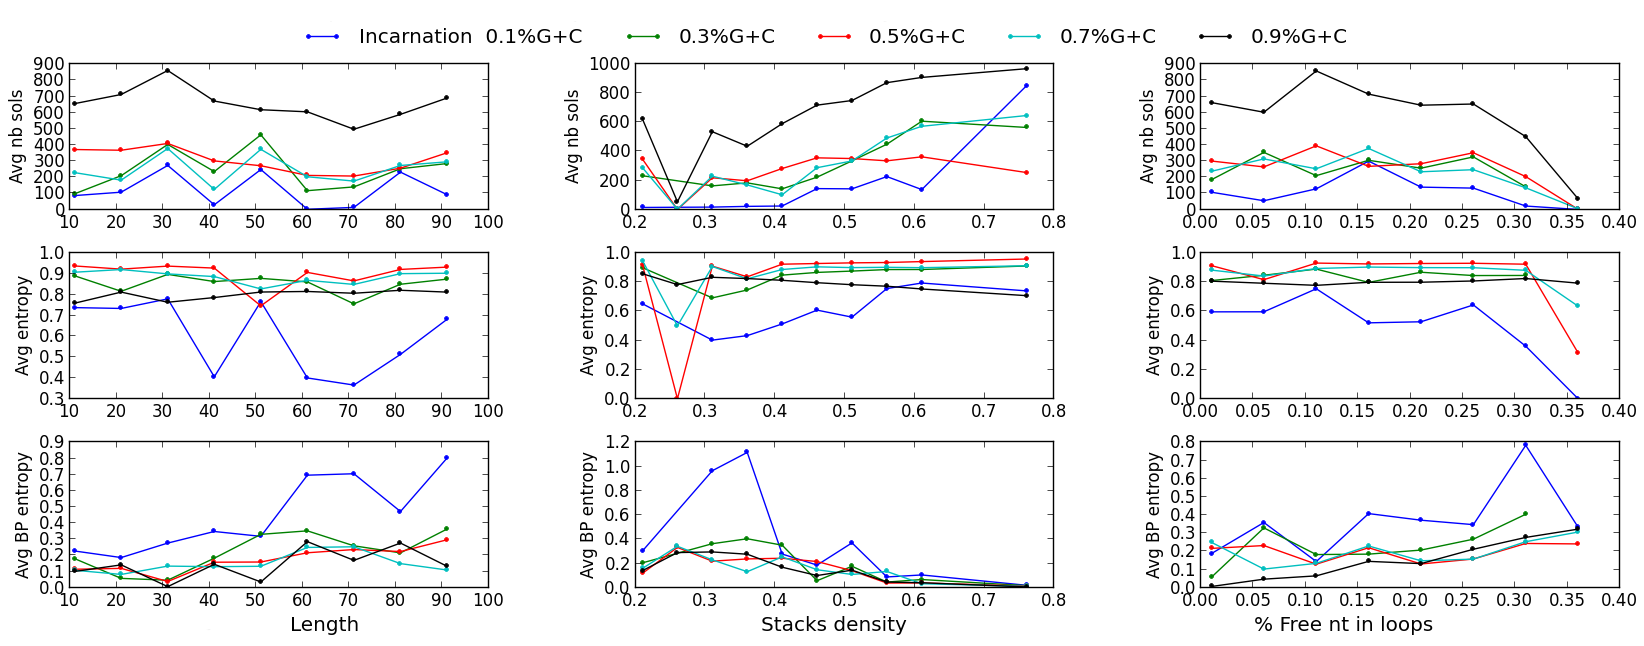
\includegraphics[scale=0.45]{Figures/nb_sols_entropy.png}
	\caption{Number of solutions generated and their average entropy. 
	The last row presents only the entropy of the nucleotides inside base 
	pairs.}
	\label{fig:nb_sols_entropy}
\end{figure}



\begin{figure}[ht!]
	\centering
	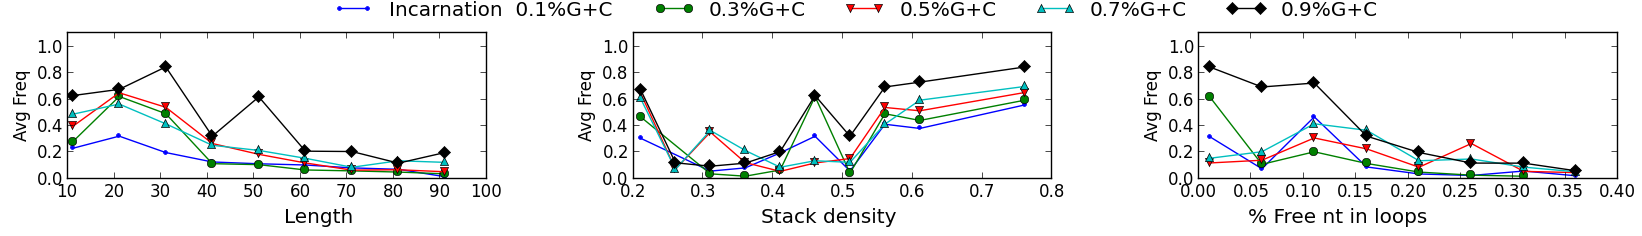
\includegraphics[scale=0.45]{Figures/freq.png}
	\caption{Average frequency of the MFE.}
	\label{fig:freq}
\end{figure}

